\section{Fibonacci Heap}
    
    Fibonacci heap serves a dual purpose
    \begin{enumerate}
        \item supports a set of operations that constitutes "mergeable heap".
        \item several fibonacci-heap operations run in constant amortized time.
    \end{enumerate}

    Fibonacci Heap is favored when the number of EXTRACT-MIN() and DELETE() is 
    relative small to the total number of operations.
    Some graphic problems have a favor on Fibonacci Heap.

    From a practical point of view, however, the constant factors and program-
ming complexity of Fibonacci heaps make them less desirable than ordinary binary
(or k-ary) heaps for most applications, except for certain applications that manage
large amounts of data.



\subsection{Supported operations and time complexity}

    Mergeable heap supports:
    \begin{enumerate}
        \item MAKE-HEAP(): create and return a new heap containing no elements
        \item INSERT(H,x): insert element x
        \item MINIMUM(H): return the pointer to the minium element in heap H
        \item EXTRACT-MIN(H):deletes the element from heap H whose key is minimum, re-
        turning a pointer to the element.
        \item UNION(H1,H2):creates and returns a new heap that contains all the elements of
        heaps H1 and H2 . Heaps H1 and H2 are “destroyed” by this operation.
    \end{enumerate}

    In addition to above operations, the Fibonacci Heap also supports:
    \begin{enumerate}
        \item DECREASE-KEY(H,x,k):assigns to element x within heap H the new key
        value k, which we assume to be no greater than its current key value.
        \item DELETE(H,x):deletes element x from heap H .
    \end{enumerate}

    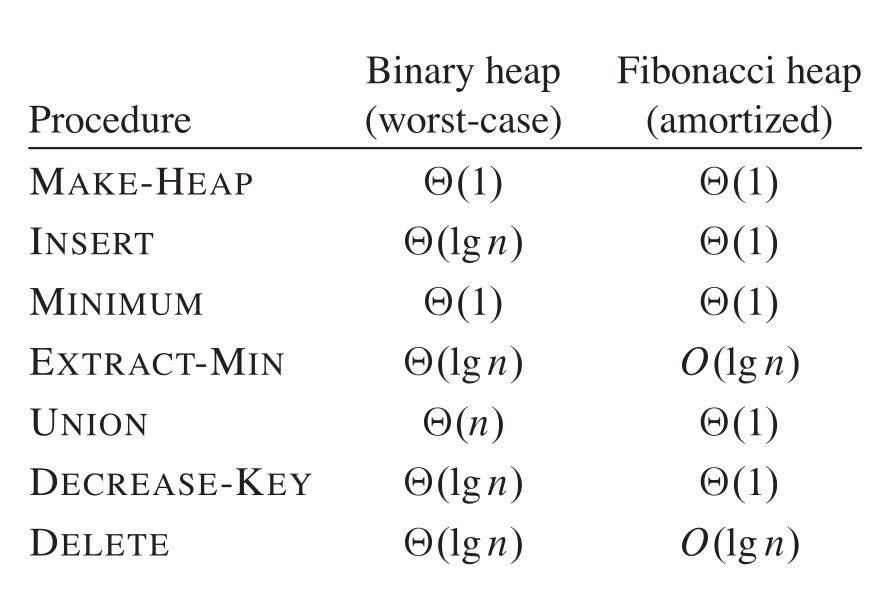
\includegraphics[width=0.5\textwidth]{contents/Advanced_Data_Structure/Fibonacci_Heap/fh_images/Screenshot from 2021-06-15 02-27-44.png}

    Note the running time of Fibonacci Heap operations are amortized.

\subsection{Structure of Fibonacci Heaps}

    \begin{enumerate}
        \item A Fibonacci Heap is a collection of rooted trees that are 
        \textbf{min-heap ordered}.
        \item Each node x contains a pointer to x.parent and a pointer x.child to
        any of its child.
        \item The children of node x are doubly-linked together in a circular. 
        The list is called \textbf{child list} of x.
        \item Each node x has x.degree what is the number of children in x's children
        list. x has x.mark indicates whether node x has lost a child since it has 
        become a child of another node. Newly created nodes are unmarked, and a node x becomes unmarked whenever it
        is made the child of another node
        \item There is H.min that points to the minimum which is also a root of tree.
        \item The roots of trees are also circular doubly-linked together, called 
        \textbf{root list}.
        \item H.n : the number of nodes inside the tree.
    \end{enumerate}

    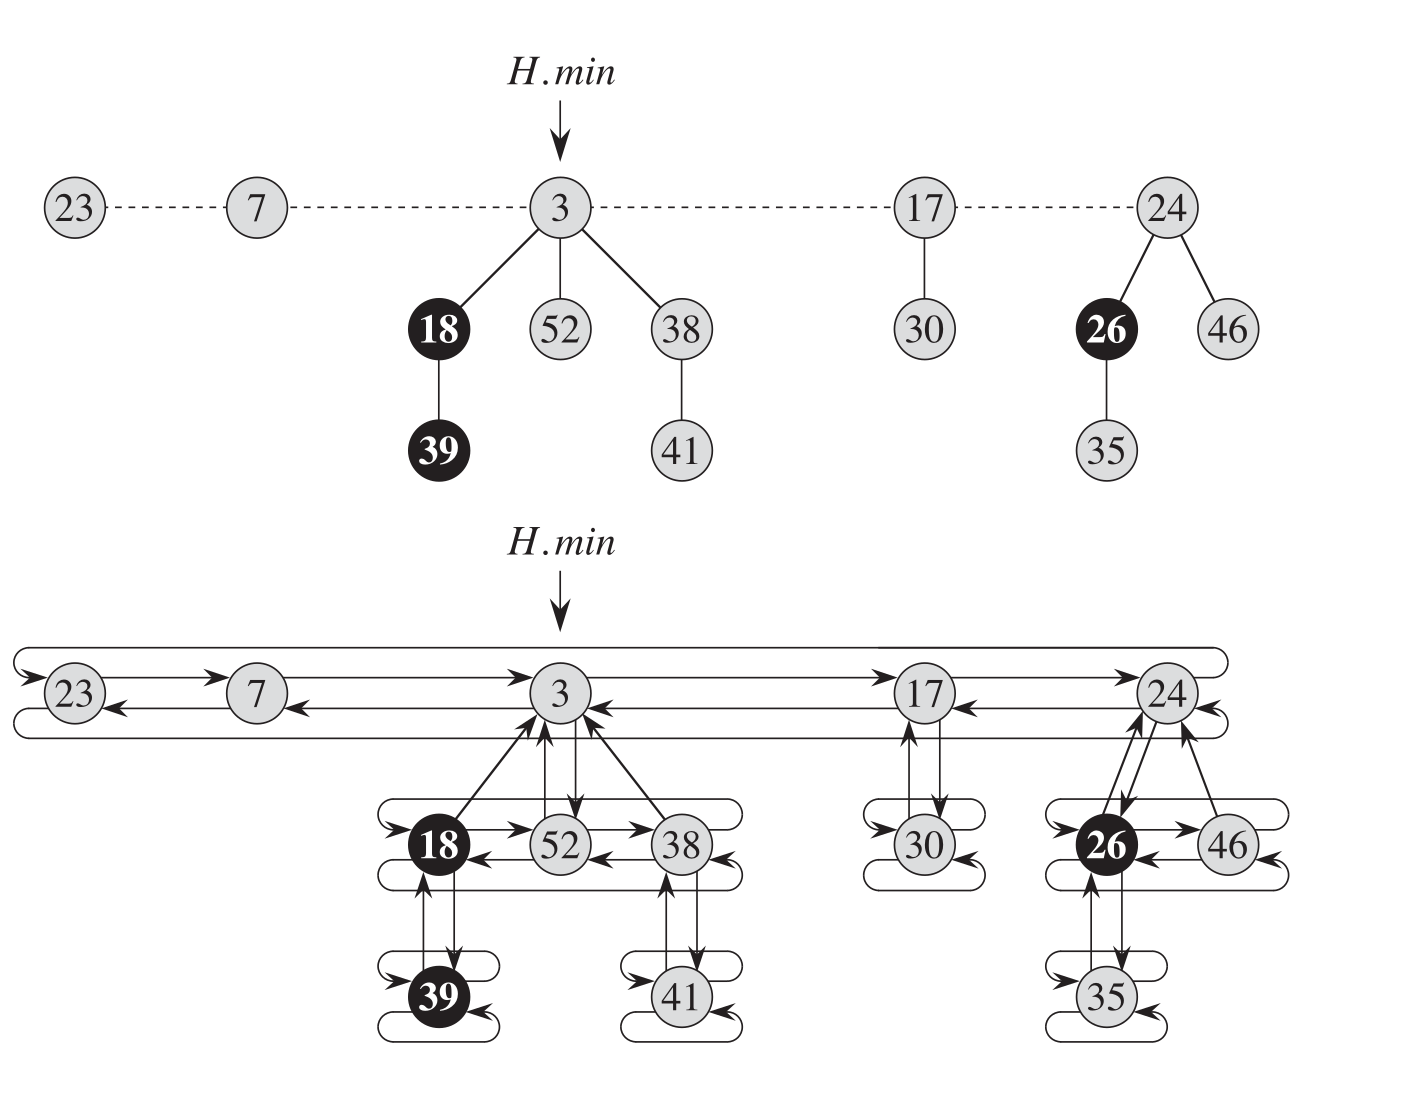
\includegraphics[width=0.7\textwidth]{contents/Advanced_Data_Structure/Fibonacci_Heap/fh_images/fb_heap_structure.png}

    In the doubly-circular-linked list, one can insert or remove a node from any location
    in O(1) time. Also, given any two CDLLs, we can concatenate them in 
    O(1) time.


\subsubsection*{Potential Function}

    t(H): the number of trees in the root list of H.

    m(H): the number of marked nodes in H.
   
    Potential Function
    \begin{equation*}
        \phi(H) = t(H) + 2m(H)
    \end{equation*}


















